\documentclass[12pt]{article}
\usepackage[T1]{fontenc}
\usepackage[T1]{polski}
\usepackage[utf8]{inputenc}
\newcommand{\BibTeX}{{\sc Bib}\TeX} 
\usepackage{graphicx}
\usepackage{amsfonts}
\usepackage{amsmath}
\usepackage{latexsym}
\usepackage{float}

\setlength{\textheight}{21cm}

\title{{\bf Zadanie nr 1 - Generacja sygnału i szumu}\linebreak
Cyfrowe Przetwarzanie Sygnałów}
\author{Dawid Jakubik, 224307 \and Hubert Gawłowski, 224298}
\date{22.04.2021}

\begin{document}
\clearpage\maketitle
\thispagestyle{empty}
\newpage
\setcounter{page}{1}
\section{Cel zadania}

Celem zadania było zapoznanie się z procesem konwersji A/C oraz C/A sygnałów jednocześnie poznając kilka metod na przeprowadzenie obu procesów jak i zaiplementowanie ich w aplikacji. 

\section{Wstęp teoretyczny}

Sygnały, które podlegaja kwantyzacji oraz rekonstrukcji generowane są na podstawie wzorów znajdujących się w instrukcji do zadania nr 1 \cite{instrukcja1}. W instrukcji \cite{instrukcja2} znajdują się wzory oraz opisy metod konwersji A/C oraz C/A użyte w celu kwantyzacji, rekonstrukcji oraz do obliczenia błędu średniokwadratowego, stosunku sygnał-szum, szczytowego stosunku sygnał-szum oraz maksymalnej różnicy.


\section{Eksperymenty i wyniki}

%%%%%%%%%%%%%%%%%%%%%%%%%%%%%%%%%%%%%%%%%%%%%%%%%%%%%%%%%%%%%%%%%%%%%%%%%%%%%%%%%%%%%%%%%%%%%%%%%%%%%%%%%%%%%%%%%
% PODROZDZIA£ PT. EKSPERYMENT NR 1 
%%%%%%%%%%%%%%%%%%%%%%%%%%%%%%%%%%%%%%%%%%%%%%%%%%%%%%%%%%%%%%%%%%%%%%%%%%%%%%%%%%%%%%%%%%%%%%%%%%%%%%%%%%%%%%%%%
W każdym z eksperymantów jako sygnał ciągły posłużył nam sygnał sinusoidalny o następujących parametrach: 
\begin{itemize}
	\item Amplituda: 4
	\item Czas początkowy: 0s
	\item Czas trwania sygnału: 2s
	\item Okres: 1s
\end{itemize}
Wygląda on następująco:
\begin{figure}[H]
    \centering
    %\includegraphics{cps_kwantyzacja_z_obcieciem.jpg}
	\includegraphics[width=\linewidth]{sygnał_sinusoidalny.jpg}
    \caption{Sygnał sinusoidalny wykorzystywany w eksperymentach}
    \label{wykres dla eksperymentu 1}
\end{figure}


\subsection{Eksperyment nr 1 Kwantyzacja równomierna z obcięciem}

Celem eksperymentu było przeprowadzenie kwantyzacji sygnału ciągłego z obcięciem.

\subsubsection{Założenia}

\begin{itemize}
    \item Częstotliwość próbkowania: 15 Hz
    \item Liczba poziomów kwantyzacji: 5
\end{itemize}
\subsubsection{Przebieg}
Skwantyzowana postać sygnału prezentuje się następująco:
\begin{figure}[H]
    \centering
    %\includegraphics{cps_kwantyzacja_z_obcieciem.jpg}
	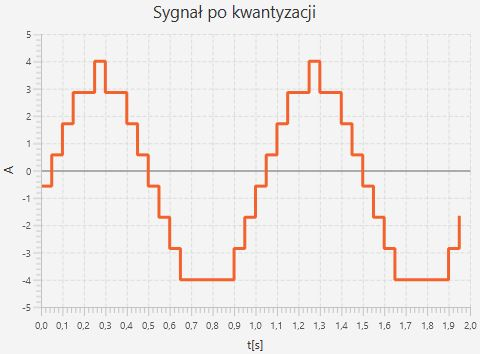
\includegraphics[width=\linewidth]{kwantyzacja_z_obcieciem.jpg}
    \caption{Kwantyzacja równomierna z obcięciem sygnału sinusoidalnego}
    \label{wykres dla eksperymentu 1.1}
\end{figure}

\subsubsection{Rezultat}
Obliczone miary dla procesu kwantyzacji:
\begin{figure}[H]
    \centering
    %\includegraphics{cps_kwantyzacja_z_obcieciem_miary.jpg}
	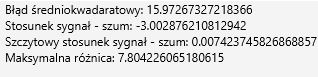
\includegraphics[width=\linewidth]{wyniki_kwantyzacja_z_obcieciem.jpg}
    \caption{Miary obliczone dla kwantyzacji równomiernej z obcięciem sygnału sinusoidalnego}
    \label{Wartości dla eksperymentu 1}
\end{figure}


%%%%%%%%%%%%%%%%%%%%%%%%%%%%%%%%%%%%%%%%%%%%%%%%%%%%%%%%%%%%%%%%%%%%%%%%%%%%%%%%%%%%%%%%%%%%%%%%%%%%%%%%%%%%%%%%%

%%%%%%%%%%%%%%%%%%%%%%%%%%%%%%%%%%%%%%%%%%%%%%%%%%%%%%%%%%%%%%%%%%%%%%%%%%%%%%%%%%%%%%%%%%%%%%%%%%%%%%%%%%%%%%%%%

\newpage
\subsection{Eksperyment nr 2 : Kwantyzacja równomierna z zaokrąglaniem}

Celem eksperymentu było przeprowadzenie kwantyzacji sygnału ciągłego z zaokrągleniem.

\subsubsection{Założenia}

\begin{itemize}
	\item Częstotliwość próbkowania: 20 Hz
	\item Liczba poziomów kwantyzacji: 8
\end{itemize}
\subsubsection{Przebieg}
Skwantyzowana postać sygnału prezentuje sie następująco:
\begin{figure}[H]
	\centering
	%\includegraphics{cps_kwantyzacja_z_zaokrągleniem.jpg}
	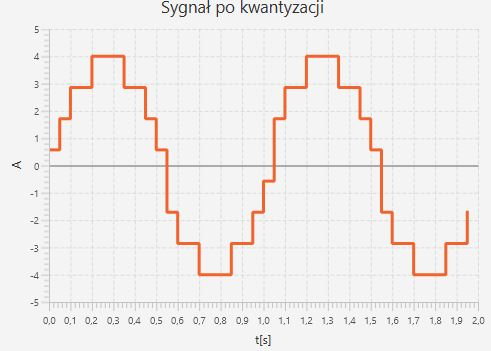
\includegraphics[width=\linewidth]{sygnal_kwantyzacja_z_zaokragleniem.jpg}
	\caption{Kwantyzacja równomierna z zaokrągleniem sygnału sinusoidalnego}
	\label{wykres dla eksperymentu 2}
\end{figure}

\subsubsection{Rezultat}
Obliczone miary dla procesu kwantyzacji:
\begin{figure}[H]
	\centering
	%\includegraphics{cps_kwantyzacja_z_zaokrągleniem_miary.jpg}
	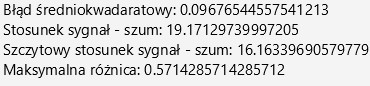
\includegraphics[width=\linewidth]{wyniki_kwantyzacja_z_zaokragleniem.jpg}
	\caption{Miary obliczone dla kwantyzacji równomiernej z zaokrągleniem sygnału sinusoidalnego}
	\label{Wartości dla eksperymentu 2}
\end{figure}


%%%%%%%%%%%%%%%%%%%%%%%%%%%%%%%%%%%%%%%%%%%%%%%%%%%%%%%%%%%%%%%%%%%%%%%%%%%%%%%%%%%%%%%%%%%%%%%%%%%%%%%%%%%%%%%%%

%%%%%%%%%%%%%%%%%%%%%%%%%%%%%%%%%%%%%%%%%%%%%%%%%%%%%%%%%%%%%%%%%%%%%%%%%%%%%%%%%%%%%%%%%%%%%%%%%%%%%%%%%%%%%%%%%
\newpage
\subsection{Eksperyment nr 3: Ekstrapolacja zerowego rzędu}


\subsubsection{Założenia}
Eksperyment nr 3 polegał na ekstrapolacji zerowego rzędu spróbkowanego sygnału ciągłego.
\subsubsection{Przebieg}
Wygenerowany sygnał prezentuje się następująco:
\begin{figure}[H]
    \centering
    %\includegraphics{cps_ekstrapolacja_0.jpg}
	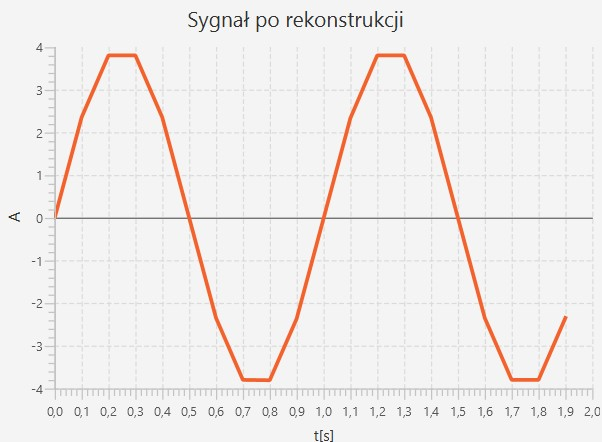
\includegraphics[width=\linewidth]{sygnal_rekonstrukcja_zero.jpg}
    \caption{Wykres Ekstrapolacji zerowego rzędu sygnału sinusoidalnego}
    \label{wykres dla eksperymentu 3}
\end{figure}



\subsubsection{Rezultat}
Obliczone parametry dla otrzymanego w rezuntacie sygnału ciągłego:
\begin{figure}[H]
    \centering
    %\includegraphics{cps_ekstrapolacja_0_miary.jpg}
	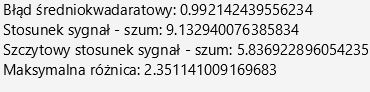
\includegraphics[width=\linewidth]{wyniki_rekonstrukcja_zero.jpg}
    \caption{Oblicznone miary dla Ekstrapolacji zerowego rzędu sygnału sinusoidalnego}
    \label{wartości dla eksperymentu 3}
\end{figure}


%%%%%%%%%%%%%%%%%%%%%%%%%%%%%%%%%%%%%%%%%%%%%%%%%%%%%%%%%%%%%%%%%%%%%%%%%%%%%%%%%%%%%%%%%%%%%%%%%%%%%%%%%%%%%%%%%

%%%%%%%%%%%%%%%%%%%%%%%%%%%%%%%%%%%%%%%%%%%%%%%%%%%%%%%%%%%%%%%%%%%%%%%%%%%%%%%%%%%%%%%%%%%%%%%%%%%%%%%%%%%%%%%%%
\newpage
\subsection{Eksperyment nr 4: Interpolacja pierwszego rzędu}

\subsubsection{Założenia}
Eksperyment nr 4 polegał na Interpolacji pierwszego rzędu spróbkowanego sygnału ciągłego.
\subsubsection{Przebieg}
Wygenerowany sygnał prezentuje się następująco:
\begin{figure}[H]
	\centering
	%\includegraphics{cps_interpolacja_1.jpg}
	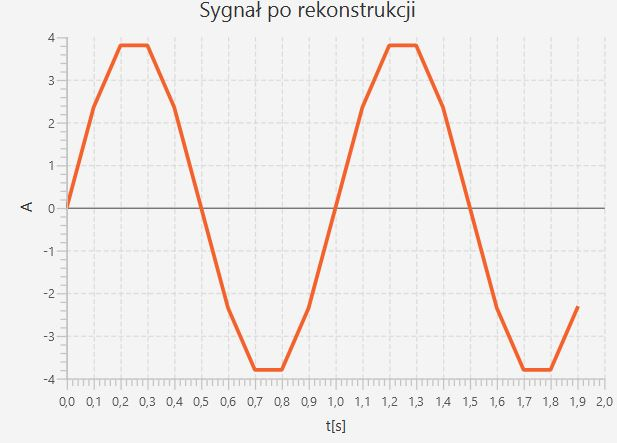
\includegraphics[width=\linewidth]{sygnal_interpolacja_pierwszy.jpg}
	\caption{Wykres Interpolacji pierwszego rzędu sygnału sinusoidalnego}
	\label{wykres dla eksperymentu 4}
\end{figure}



\subsubsection{Rezultat}
Obliczone parametry dla otrzymanego w rezultacie sygnału ciągłego:
\begin{figure}[H]
	\centering
	%\includegraphics{cps_interpolacja_1_miary.jpg}
	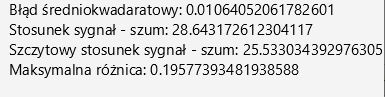
\includegraphics[width=\linewidth]{wyniki_interpolacja_pierwszy.jpg}
	\caption{Oblicznone miary dla Interpolacja pierwszego rzędu sygnału sinusoidalnego}
	\label{wartości dla eksperymentu 4}
\end{figure}

%%%%%%%%%%%%%%%%%%%%%%%%%%%%%%%%%%%%%%%%%%%%%%%%%%%%%%%%%%%%%%%%%%%%%%%%%%%%%%%%%%%%%%%%%%%%%%%%%%%%%%%%%%%%%%%%%

%%%%%%%%%%%%%%%%%%%%%%%%%%%%%%%%%%%%%%%%%%%%%%%%%%%%%%%%%%%%%%%%%%%%%%%%%%%%%%%%%%%%%%%%%%%%%%%%%%%%%%%%%%%%%%%%%
\newpage
\subsection{Eksperyment nr 5: Rekonstrukcja w oparciu o funkcję sinc }
\subsubsection{Założenia}
Eksperyment nr 3 polegał na rekonstrukcji w oparciu o funkcję sinc spróbkowanego sygnału ciągłego.
\subsubsection{Przebieg}
Wygenerowany sygnał prezentuje się następująco:
\begin{figure}[H]
	\centering
	%\includegraphics{cps_rekonstrukcja_sinc.jpg}
	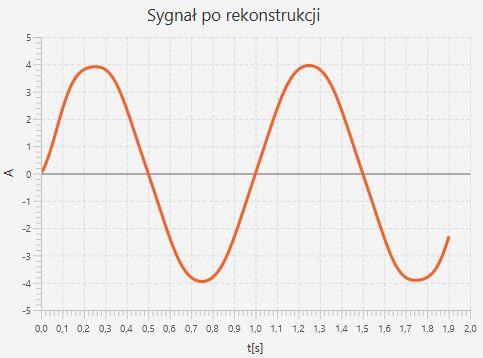
\includegraphics[width=\linewidth]{sygnal_sinc.jpg}
	\caption{Wykres rekonstrukcji w oparciu o funkcję sinc sygnału sinusoidalnego}
	\label{wykres dla eksperymentu 5}
\end{figure}



\subsubsection{Rezultat}
Obliczone parametry dla otrzymanego w rezuntacie sygnału ciągłego:
\begin{figure}[H]
	\centering
	%\includegraphics{cps_rekonstrukcja_sincmiary.jpg}
	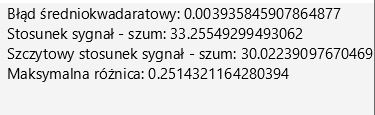
\includegraphics[width=\linewidth]{wyniki_sinc.jpg}
	\caption{Oblicznone miary dla rekonstrukcji w oparciu o funkcję sinc sygnału sinusoidalnego}
	\label{wartości dla eksperymentu 5}
\end{figure}
%%%%%%%%%%%%%%%%%%%%%%%%%%%%%%%%%%%%%%%%%%%%%%%%%%%%%%%%%%%%%%%%%%%%%%%%%%%%%%%%%%%%%%%%%%%%%%%%%%%%%%%%%%%%%%%%%

%%%%%%%%%%%%%%%%%%%%%%%%%%%%%%%%%%%%%%%%%%%%%%%%%%%%%%%%%%%%%%%%%%%%%%%%%%%%%%%%%%%%%%%%%%%%%%%%%%%%%%%%%%%%%%%%%

\section{Wnioski}
\begin{itemize}
    \item Każdy sygnał ciągły można zdyskretyzować poprzez próbkowanie a następnie te próbki skwantyzować by ograniczyć dokładność zapisu oraz ilość pamięci potrzebnej do zapisu sygnału zdyskrekretyzowanego.
    \item Program poprawnie kwantyzuje oraz rekonstruuje sygnały.
    \item Program pozwala obliczenie 4 miar dla każdego skwantyzowanego sygnału.
    \item Najbardziej przypominający kształtem sygnał zrekonstruowany powstaje po rekonstrukcji z wykorzystaniem funkcji sinc.
    \item Kwantyzacja pozwala w efektywny sposób przedstawić sygnał w postaci cyfrowej
    \item Im większa częstotliwość próbkowania, tym jakość rekonstrukcji jest lepsza
    \item Im więcej więcej poziomów kwantyzacji, tym błąd kwantyzacji jest mniejszy.
\end{itemize}
 

%%%%%%%%%%%%%%%%%%%%%%%%%%%%%%%%%%%%%%%%%%%%%%%%%%%%%%%%%%%%%%%%%%%%%%%%%%%%%%%%%%%%%%%%%%%%%%%%%%%%%%%%%%%%%%%%%
% BIBLIOGRAFIA
%%%%%%%%%%%%%%%%%%%%%%%%%%%%%%%%%%%%%%%%%%%%%%%%%%%%%%%%%%%%%%%%%%%%%%%%%%%%%%%%%%%%%%%%%%%%%%%%%%%%%%%%%%%%%%%%%
\begin{thebibliography}{}
\bibitem{instrukcja1} Instrukcja do zadania 1 na stronie przedmiotu. [przeglądany 28.04.2021], Dostępny w: https://ftims.edu.p.lodz.pl/file.php/154/zadanie120101011.pdf
\bibitem{instrukcja2} Instrukcja do zadania 2 na stronie przedmiotu. [przeglądany 28.04.2021], Dostępny w: {https://ftims.edu.p.lodz.pl/pluginfile.php/13449/modresource/content/0/zadanie2.pdf}

\end{thebibliography}



\end{document}
